\chapter{Evaluierung}

Die Qualität der Ergebnisse des in der Implementierung realisierten Modells wird in diesem Kapitel durch ein Testexperiment überprüft. Weiterhin werden Ausführungszeiten für beispielsweise verschieden große $k$ beim Bag of Visual Words betrachtet, um eine Einsicht in die Performance der Algorithmen zu gewinnen.
Im Kapitel Experimentaufbau wird zunächst das Experiement sowie verwendete Metriken und Ergebnistypen behandelt. Nachfolgend wird erläutert, wie die großen Menge an benötigten Trainings- und Testdaten wiederholbar und automatisiert aufgebaut wird. Dieser Abschnitt illustriert auch, wie eine Durchführung des Experiments vonstattengeht. Im letzten Teil werden dann konkrete Testgruppen aus den Caltech101 \cite{cal2004} Bilddaten erzeugt. Diese Menge an Bilddaten hat große Verbreitung im Bereich der Objekterkennung gefunden. Auf diese Weise ist ein Vergleich mit Arbeiten Anderer prinzipiell möglich.

\section{Testdaten und Testgenerierung}

Der Abschnitt Testdaten stellt die hier verwendete Menge von Bildern vor, die Caltech101, welche extra für den Test von Algorithmen bezüglich der Objekterkennung in Bildern entwickelt wurde.\newline
Im Folgenden Abschnitt zur Testgenerierung wird ein Verfahren zur zufälligen Auswahl von Trainings- und Testbildern unter Berücksichtigung verschiedener Restriktionen, wie z.B. dem Verhältnis der Anzahl von Trainings- zu Testbildern vorgestellt.

\subsection{Testdaten}

Als Testmenge wurden die Bilder der Caltech101 Menge verwendet. Bei Caltech101 handelt es sich um eine weit verbreitete Menge von Bilddaten, die vorwiegend zum Test von Algorithmen bezüglich der Objekterkennung in Bildern dient. Insgesamt liegen, wie der Name sagt, 101 Kategorien vor, die jeweils zwischen 40 und 800 Bildern enthalten. Auf der offiziellen Webseite \footnote{http://www.vision.caltech.edu/Image\textunderscore Datasets/Caltech101/} und im Artikel der Autoren wir empfohlen, die eigene Arbeit mit derer anderen vergleichbar zu halten, indem:

\begin{itemize}
	\item Eine feste Anzahl an Trainings- und Testbildern verwendet wird.
	\item Experimente mit einer zufälligen Auswahl an Bildern wiederholt werden.
	\item Ähnlich viele Bilder, wie in den Arbeiten anderer, verwendet werden (1, 3, 5, 10, 15, 20 oder 30 Trainingsbilder; 20 oder 30 Testbilder).
\end{itemize}

Abbildung \ref{img:strawberries} zeigt vier Bilder aus der Kategorie \enquote{Erdbeere}. Neben Bildern von realen Rosengewächsen sind auch Zeichnungen und Objekte enthalten, die Form und Farbe der Erdbeere nachempfunden sind. Auch sind die Objekte auf einem Bild zum Teil in unterschiedlicher Menge vorhanden. Durch dies Variation ist ein Algorithmus so gefordert, tatsächlich eine Abstraktion zu lernen.

\begin{figure}
	\centering
	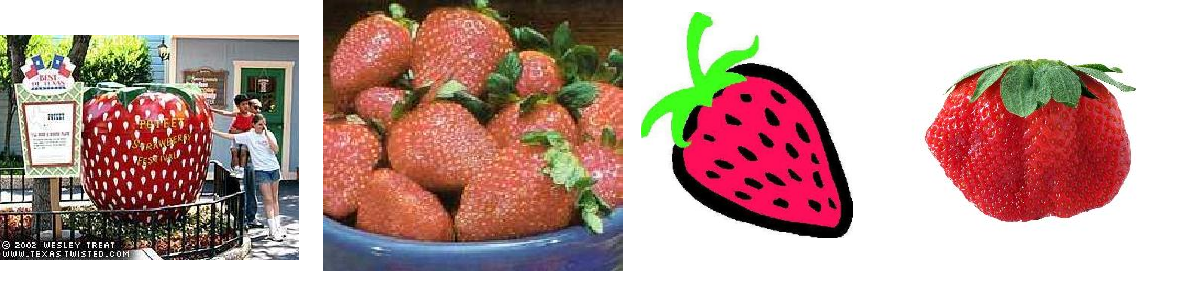
\includegraphics[scale=0.5]{images/strawberry.png}
	\caption{Verschiedene Bilder aus der Kategorie \enquote{Erdbeere} der Caltech101 Bilddaten.}
	\label{img:strawberries}
\end{figure}

Die Caltech101 Daten liegen nach Download kategorisiert im JPG-Format vor. Die Struktur wurde so beibehalten und ist noch für die Testgenerierung relevant. Direkt unter dem Caltech101-Ordner ist pro Kategorie ein Ordner vorhanden, der die jeweiligen Bilder immer im gleichen Namensschema enthält:\newline

\dirtree{%src
.1 Caltech101.
.2 accordion.
.3 image\textunderscore 0001.jpg.
.3 image\textunderscore 0002.jpg.
.3 ....
.2 airplanes.
.3 ....
.2 ....
}

\subsection{Testgenerierung}

Die Generierung von Testdaten bietet sich aus mehreren Gründen an. Zum einen sind enorm viele Trainingsdaten notwendig, um ein leistungsfähiges Modell zu generieren. Zum anderen sollen im Test ca. 2000 Bildpaare verwendet werden. Ein manueller Testaufbau wäre fehleranfällig und nicht sehr flexibel. Da ein praktisch taugliches Modell erst durch die Variation einiger Parameter gefunden werden kann, ist es wünschenswert, Testdaten mit verschiedenen Eigenschaften generieren zu können:

\begin{itemize}
	\item Die Anzahl der Kategorien sollte bestimmbar sein. Dies entspricht einer Kategorie der Caltech101 Daten. Somit sind hier theoretisch bis zu 101 Kategorien im Test denkbar.
	\item Das Verhältnis bzw. Die Anzahl an Trainings- und Testbildern muss definierbar sein.
\end{itemize}

Letztendlich sollen die Histogramme der \textit{Visual Words} zweier Bilder miteinander verglichen und so die Ähnlichkeit gemessen werden. Ein Programm automatisiert daher die Generierung solcher Paare: Es werden zufällige Bildpaare aus ausgewählten Kategorien (\textit{airplanes}, \textit{anchor}, ...) selektiert. Diese Paare, sowie die Information, ob die Bilder in der selben oder einer verschiedenen Kategorie liegen, stellen einen Testkandidaten dar. Zwei Bilder liegen dabei in der selben Klasse, wenn sie im selben Ordner im Dateisystem, also hier im Caltech101-Ordner, enthalten sind. Das Ergebnis wird dann als Datei \textit{test \textunderscore time.txt} gespeichert. Die Pfade der Bilder werden hierbei relativ zum Caltech101-Ordner gespeichert, die Information über die Kategorie wird als \enquote{+} bzw. \enquote{-} kodiert. Eine Datei für die Kategorien \textit{airplanes} und \textit{anchor} könnte dann so beginnen:\newline

\begin{lstlisting}
airplanes/image_0023.jpg airplanes/image_0009.jpg +
airplanes/image_0002.jpg anchor/image_0015.jpg -
anchor/image_0013.jpg airplanes/image_0002.jpg -
anchor/image_0001.jpg anchor/image_0005.jpg +
airplanes/image_0006.jpg anchor/image_0006.jpg -
...
\end{lstlisting}

Neben den zu verwendenden Kategorien muss bei Erzeugung die Anzahl der Testkandidaten, das Verhältnis von positiven zu negativen Kategorien sowie die Anzahl der Trainings- und Testbilder angegeben werden. \newline
Die Bilder, welche durch das Programm für das Training ausgewählt wurden, werden separat als \textit{train\textunderscore time.txt} gespeichert. Pro Zeile ist hier der relative Pfad des Bildes innerhalb des Caltech101-Ordners enthalten.
\todo{Neu Aufrufer erwähnen}

\section{Experimentaufbau}

Das Experiment soll sowohl die Feature-Kompression durch einen Autoencoder testen als auch die Kategorisierung bzw. den Vergleich der Bilder durch den Bag of Visual Words. Aus diesem Grund ist das Experiment zweigeteilt: 

\begin{enumerate}[(a)]%
	\item In dieser Variante findet ein reiner Test des Bag of Visual Words statt. Hierfür werden durch SIFT die Feature-Deskriptoren von Trainingsbildern extrahiert und direkt als Eingabe an den Bag of Visual Words gegeben. Anschließend folgt die Verarbeitung der Testbilder.
	\item Hier wird nach Extraktion der \textit{keypoints} durch den SIFT-Detektor der Feature-Deskriptor durch den Autoencoder erzeugt. Die so erhaltenen Features werden dann wie in \textbf{(a)} durch den Bag of Visual Words gruppiert und anschließend die \textit{Visual Words} der Testbilder erzeugt.
\end{enumerate}

Wichtig ist, dass pro Durchführung des Experiments in beiden Varianten die gleichen Trainings- und Testbilder verwendet werden, damit die Deskriptoren miteinander vergleichbar sind. \newline
\todo{Vergleich Bilder Distanzmetrik} Für jede werden nun die jeweiligen\textit{Visual Words} ermittelt und anhand der euklidischen Distanz verglichen. 

Hier gibt es zwei Fälle zu unterscheiden:

\begin{itemize}
	\item \textbf{True Positives} Bei \textit{True Positives} handelt es sich um zwei Bildern die entweder in der gleichen oder einer verschiedenen Klasse liegen und die Vorhersage des Modells diesbezüglich korrekt ist.
	\item \textbf{False Positives} Auch hier liegen die Testbilder in der gleichen oder einer verschiedenen Klasse, die Vorhersage durch das Modell ist jedoch nicht korrekt.
\end{itemize}

Damit ein Modell zuverlässige Ergebnisse liefert, muss es größtenteils \textit{True Positives} erkennen, bzw. der Anteil der \textit{True Positives} sollte im Verhältnis zu den \textit{False Positives} bei weitem überwiegen. Für eine visuelle Darstellung dieses Verhältnisses eignet sich die \textit{Receiver Operating Characteristic (ROC)}: Diese stellt für verschiedene Parameter die \textit{True Positives} auf der Ordinate und die \textit{False-Positives} auf der Abzisse dar, sodass der optimale Parameter anhand der resultierenden Kurve abgelesen werden kann.

\section{Experimentdurchführung}

\todo{LALALA}